\documentclass[8pt,aspectratio=169]{beamer}
\usetheme{Madrid}
\usepackage{graphicx}
\usepackage{booktabs}
\usepackage{adjustbox}
\usepackage{multicol}
\usepackage{amsmath}
\usepackage{amssymb}
\usepackage{listings}
\usepackage{xcolor}

% Color definitions
\definecolor{mlblue}{RGB}{0,102,204}
\definecolor{mlpurple}{RGB}{51,51,178}
\definecolor{mllavender}{RGB}{173,173,224}
\definecolor{mllavender2}{RGB}{193,193,232}
\definecolor{mllavender3}{RGB}{204,204,235}
\definecolor{mllavender4}{RGB}{214,214,239}
\definecolor{mlorange}{RGB}{255, 127, 14}
\definecolor{mlgreen}{RGB}{44, 160, 44}
\definecolor{mlred}{RGB}{214, 39, 40}
\definecolor{mlgray}{RGB}{127, 127, 127}

% Additional colors for template compatibility
\definecolor{lightgray}{RGB}{240, 240, 240}
\definecolor{midgray}{RGB}{180, 180, 180}

% Solidity colors
\definecolor{solkeyword}{RGB}{0,102,153}
\definecolor{solstring}{RGB}{163,21,21}
\definecolor{solcomment}{RGB}{0,128,0}
\definecolor{solnumber}{RGB}{0,128,128}

% Solidity language definition
\lstdefinelanguage{Solidity}{
  keywords={pragma, solidity, contract, function, public, private, external, internal, view, pure, payable, returns, return, if, else, for, while, mapping, address, uint, uint256, int, string, bool, bytes, bytes32, event, emit, modifier, require, constructor, memory, storage, calldata, msg, sender, value, this, new, delete, true, false},
  keywordstyle=\color{solkeyword}\bfseries,
  sensitive=true,
  comment=[l]{//},
  morecomment=[s]{/*}{*/},
  commentstyle=\color{solcomment}\ttfamily,
  stringstyle=\color{solstring}\ttfamily,
  morestring=[b]',
  morestring=[b]"
}

% Apply custom colors to Madrid theme
\setbeamercolor{palette primary}{bg=mllavender3,fg=mlpurple}
\setbeamercolor{palette secondary}{bg=mllavender2,fg=mlpurple}
\setbeamercolor{palette tertiary}{bg=mllavender,fg=white}
\setbeamercolor{palette quaternary}{bg=mlpurple,fg=white}
\setbeamercolor{structure}{fg=mlpurple}
\setbeamercolor{section in toc}{fg=mlpurple}
\setbeamercolor{subsection in toc}{fg=mlblue}
\setbeamercolor{title}{fg=mlpurple}
\setbeamercolor{frametitle}{fg=mlpurple,bg=mllavender3}
\setbeamercolor{block title}{bg=mllavender2,fg=mlpurple}
\setbeamercolor{block body}{bg=mllavender4,fg=black}

\setbeamertemplate{navigation symbols}{}
\setbeamertemplate{itemize items}[circle]
\setbeamertemplate{enumerate items}[default]
\setbeamersize{text margin left=5mm,text margin right=5mm}

\newcommand{\bottomnote}[1]{%
\vfill
\vspace{-2mm}
\textcolor{mllavender2}{\rule{\textwidth}{0.4pt}}
\vspace{1mm}
\footnotesize
\textbf{#1}
}

% TikZ and pgfplots packages
\usepackage{tikz}
\usepackage{pgfplots}
\pgfplotsset{compat=1.18}
\usetikzlibrary{arrows.meta, positioning, shapes.geometric, shapes.symbols, calc, decorations.pathmorphing, mindmap}

\title{DAOs \& Governance: A Visual Introduction}
\subtitle{Standalone Mini-Lecture}
\author{Prof.~Dr.~Joerg Osterrieder}
\institute{University Lecture Series}
\date{\today}
\begin{document}

% Frame 1: Title
\begin{frame}[plain]
\vspace{2cm}
\begin{center}
{\Huge\color{mlpurple} DAOs \& Governance: A Visual Introduction}\\[0.4cm]
{\Large\color{mlblue} Standalone Mini-Lecture}\\[0.3cm]
\textcolor{mlgray}{\rule{6cm}{0.4pt}}\\[0.3cm]
{\small\itshape ``The future of organization is decentralized'' -- Vitalik Buterin}\\[1.5cm]
{\normalsize Prof.~Dr.~Joerg Osterrieder}\\[0.2cm]
{\small University Lecture Series}\\[0.2cm]
{\small \today}
\end{center}

\bottomnote{This mini-lecture covers Decentralized Autonomous Organizations: how they work, governance mechanisms, treasury management, attacks, and real-world examples.}
\end{frame}

% Frame 2: What is a DAO?
\begin{frame}{What is a DAO?}
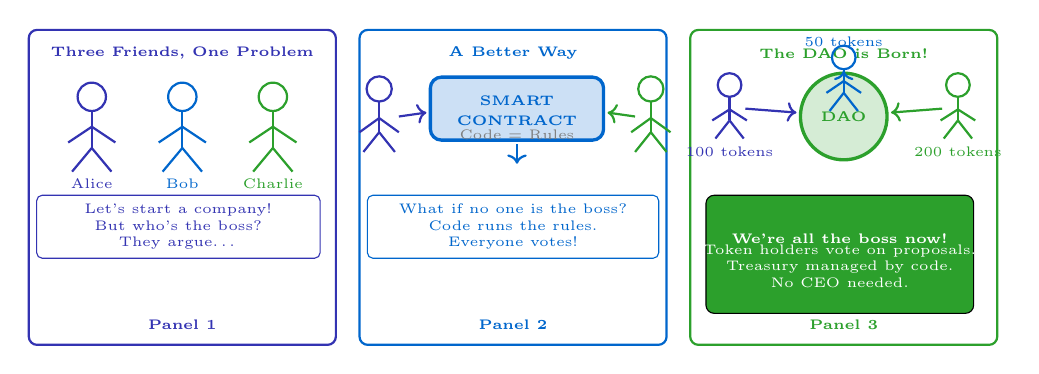
\begin{tikzpicture}
  % Panel borders
  \draw[thick, mlpurple, rounded corners=3pt] (0.1,0.2) rectangle (4.0,4.2);
  \draw[thick, mlblue,   rounded corners=3pt] (4.3,0.2) rectangle (8.2,4.2);
  \draw[thick, mlgreen,  rounded corners=3pt] (8.5,0.2) rectangle (12.4,4.2);

  % --- Panel 1: Alice, Bob, Charlie want to pool money ---
  \node[font=\tiny\bfseries, mlpurple] at (2.05,3.9) {Three Friends, One Problem};
  % Alice stick figure
  \draw[mlpurple,thick] (0.9,3.35) circle (0.18);
  \draw[mlpurple,thick] (0.9,3.17) -- (0.9,2.70);
  \draw[mlpurple,thick] (0.9,2.97) -- (0.6,2.77);
  \draw[mlpurple,thick] (0.9,2.97) -- (1.2,2.77);
  \draw[mlpurple,thick] (0.9,2.70) -- (0.65,2.40);
  \draw[mlpurple,thick] (0.9,2.70) -- (1.15,2.40);
  \node[font=\tiny, mlpurple] at (0.9,2.25) {Alice};
  % Bob stick figure
  \draw[mlblue,thick] (2.05,3.35) circle (0.18);
  \draw[mlblue,thick] (2.05,3.17) -- (2.05,2.70);
  \draw[mlblue,thick] (2.05,2.97) -- (1.75,2.77);
  \draw[mlblue,thick] (2.05,2.97) -- (2.35,2.77);
  \draw[mlblue,thick] (2.05,2.70) -- (1.80,2.40);
  \draw[mlblue,thick] (2.05,2.70) -- (2.30,2.40);
  \node[font=\tiny, mlblue] at (2.05,2.25) {Bob};
  % Charlie stick figure
  \draw[mlgreen,thick] (3.2,3.35) circle (0.18);
  \draw[mlgreen,thick] (3.2,3.17) -- (3.2,2.70);
  \draw[mlgreen,thick] (3.2,2.97) -- (2.9,2.77);
  \draw[mlgreen,thick] (3.2,2.97) -- (3.5,2.77);
  \draw[mlgreen,thick] (3.2,2.70) -- (2.95,2.40);
  \draw[mlgreen,thick] (3.2,2.70) -- (3.45,2.40);
  \node[font=\tiny, mlgreen] at (3.2,2.25) {Charlie};
  % Speech bubble
  \draw[fill=white, draw=mlpurple, rounded corners=2pt] (0.2,1.3) rectangle (3.8,2.1);
  \node[font=\tiny, mlpurple, align=center] at (2.0,1.7) {Let's start a company!\\But who's the boss?\\They argue\ldots};
  \node[font=\tiny\bfseries, mlpurple] at (2.05,0.45) {Panel 1};

  % --- Panel 2: They discover DAOs ---
  \node[font=\tiny\bfseries, mlblue] at (6.25,3.9) {A Better Way};
  % Smart contract box at center
  \draw[fill=mlblue!20, draw=mlblue, very thick, rounded corners=4pt] (5.2,2.8) rectangle (7.4,3.6);
  \node[font=\tiny\bfseries, mlblue, align=center] at (6.3,3.3) {SMART};
  \node[font=\tiny\bfseries, mlblue, align=center] at (6.3,3.05) {CONTRACT};
  \node[font=\tiny, mlgray, align=center] at (6.3,2.87) {Code = Rules};
  % Arrows from figures to contract
  \draw[->, thick, mlpurple] (4.8,3.1) -- (5.15,3.15);
  \draw[->, thick, mlblue]   (6.3,2.75) -- (6.3,2.50);
  \draw[->, thick, mlgreen]  (7.8,3.1) -- (7.45,3.15);
  % Alice left
  \draw[mlpurple,thick] (4.55,3.45) circle (0.16);
  \draw[mlpurple,thick] (4.55,3.29) -- (4.55,2.90);
  \draw[mlpurple,thick] (4.55,3.08) -- (4.3,2.90);
  \draw[mlpurple,thick] (4.55,3.08) -- (4.8,2.90);
  \draw[mlpurple,thick] (4.55,2.90) -- (4.35,2.65);
  \draw[mlpurple,thick] (4.55,2.90) -- (4.75,2.65);
  % Charlie right
  \draw[mlgreen,thick] (8.0,3.45) circle (0.16);
  \draw[mlgreen,thick] (8.0,3.29) -- (8.0,2.90);
  \draw[mlgreen,thick] (8.0,3.08) -- (7.75,2.90);
  \draw[mlgreen,thick] (8.0,3.08) -- (8.25,2.90);
  \draw[mlgreen,thick] (8.0,2.90) -- (7.80,2.65);
  \draw[mlgreen,thick] (8.0,2.90) -- (8.20,2.65);
  % Speech bubble
  \draw[fill=white, draw=mlblue, rounded corners=2pt] (4.4,1.3) rectangle (8.1,2.1);
  \node[font=\tiny, mlblue, align=center] at (6.25,1.7) {What if no one is the boss?\\Code runs the rules.\\Everyone votes!};
  \node[font=\tiny\bfseries, mlblue] at (6.25,0.45) {Panel 2};

  % --- Panel 3: They create a DAO ---
  \node[font=\tiny\bfseries, mlgreen] at (10.45,3.9) {The DAO is Born!};
  % DAO circle
  \draw[fill=mlgreen!20, draw=mlgreen, very thick] (10.45,3.1) circle (0.55);
  \node[font=\tiny\bfseries, mlgreen, align=center] at (10.45,3.1) {DAO};
  % Token holders
  \draw[mlpurple,thick] (9.0,3.5) circle (0.15);
  \draw[mlpurple,thick] (9.0,3.35) -- (9.0,3.05);
  \draw[mlpurple,thick] (9.0,3.19) -- (8.78,3.05);
  \draw[mlpurple,thick] (9.0,3.19) -- (9.22,3.05);
  \draw[mlpurple,thick] (9.0,3.05) -- (8.82,2.82);
  \draw[mlpurple,thick] (9.0,3.05) -- (9.18,2.82);
  \draw[->, thick, mlpurple] (9.2,3.2) -- (9.85,3.15);
  \node[font=\tiny, mlpurple] at (9.0,2.65) {100 tokens};
  \draw[mlblue,thick] (10.45,3.85) circle (0.15);
  \draw[mlblue,thick] (10.45,3.7) -- (10.45,3.4);
  \draw[mlblue,thick] (10.45,3.55) -- (10.23,3.4);
  \draw[mlblue,thick] (10.45,3.55) -- (10.67,3.4);
  \draw[mlblue,thick] (10.45,3.4) -- (10.27,3.17);
  \draw[mlblue,thick] (10.45,3.4) -- (10.63,3.17);
  \draw[->, thick, mlblue] (10.45,3.67) -- (10.45,3.68);
  \node[font=\tiny, mlblue] at (10.45,4.05) {50 tokens};
  \draw[mlgreen,thick] (11.9,3.5) circle (0.15);
  \draw[mlgreen,thick] (11.9,3.35) -- (11.9,3.05);
  \draw[mlgreen,thick] (11.9,3.19) -- (11.68,3.05);
  \draw[mlgreen,thick] (11.9,3.19) -- (12.12,3.05);
  \draw[mlgreen,thick] (11.9,3.05) -- (11.72,2.82);
  \draw[mlgreen,thick] (11.9,3.05) -- (12.08,2.82);
  \draw[->, thick, mlgreen] (11.7,3.2) -- (11.05,3.15);
  \node[font=\tiny, mlgreen] at (11.9,2.65) {200 tokens};
  % Result box
  \draw[fill=mlgreen, rounded corners=3pt] (8.7,0.6) rectangle (12.1,2.1);
  \node[font=\tiny\bfseries, white, align=center] at (10.4,1.55) {We're all the boss now!};
  \node[font=\tiny, white, align=center] at (10.4,1.2) {Token holders vote on proposals.\\Treasury managed by code.\\No CEO needed.};
  \node[font=\tiny\bfseries, mlgreen] at (10.45,0.45) {Panel 3};
\end{tikzpicture}

\bottomnote{DAO = Decentralized Autonomous Organization. Smart contracts replace management: rules are encoded in code, decisions made by token-weighted voting.}
\end{frame}

% Frame 3: Traditional Org vs DAO
\begin{frame}{Traditional Organization vs.\ DAO}
\begin{columns}[c]
  \begin{column}{0.48\textwidth}
    \centering
    {\small\bfseries\color{mlred} Traditional Hierarchy}\\[0.2cm]
    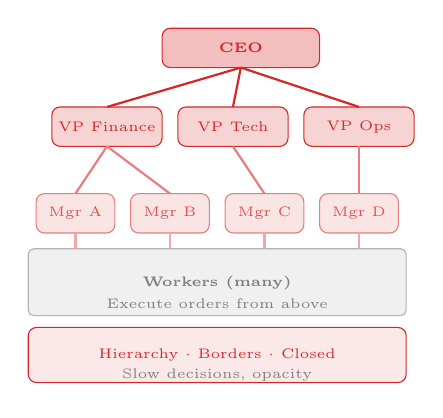
\begin{tikzpicture}
      % CEO
      \draw[fill=mlred!30, draw=mlred, rounded corners=3pt] (1.8,4.5) rectangle (3.8,5.0);
      \node[font=\tiny\bfseries, mlred, align=center] at (2.8,4.75) {CEO};
      % VP level
      \draw[fill=mlred!20, draw=mlred, rounded corners=3pt] (0.4,3.5) rectangle (1.8,4.0);
      \node[font=\tiny, mlred, align=center] at (1.1,3.75) {VP Finance};
      \draw[fill=mlred!20, draw=mlred, rounded corners=3pt] (2.0,3.5) rectangle (3.4,4.0);
      \node[font=\tiny, mlred, align=center] at (2.7,3.75) {VP Tech};
      \draw[fill=mlred!20, draw=mlred, rounded corners=3pt] (3.6,3.5) rectangle (5.0,4.0);
      \node[font=\tiny, mlred, align=center] at (4.3,3.75) {VP Ops};
      % Connecting lines CEO to VPs
      \draw[thick, mlred] (2.8,4.5) -- (1.1,4.0);
      \draw[thick, mlred] (2.8,4.5) -- (2.7,4.0);
      \draw[thick, mlred] (2.8,4.5) -- (4.3,4.0);
      % Manager level
      \draw[fill=mlred!12, draw=mlred!60, rounded corners=3pt] (0.2,2.4) rectangle (1.2,2.9);
      \node[font=\tiny, mlred!80, align=center] at (0.7,2.65) {Mgr A};
      \draw[fill=mlred!12, draw=mlred!60, rounded corners=3pt] (1.4,2.4) rectangle (2.4,2.9);
      \node[font=\tiny, mlred!80, align=center] at (1.9,2.65) {Mgr B};
      \draw[fill=mlred!12, draw=mlred!60, rounded corners=3pt] (2.6,2.4) rectangle (3.6,2.9);
      \node[font=\tiny, mlred!80, align=center] at (3.1,2.65) {Mgr C};
      \draw[fill=mlred!12, draw=mlred!60, rounded corners=3pt] (3.8,2.4) rectangle (4.8,2.9);
      \node[font=\tiny, mlred!80, align=center] at (4.3,2.65) {Mgr D};
      % Lines VPs to Managers
      \draw[thick, mlred!60] (1.1,3.5) -- (0.7,2.9);
      \draw[thick, mlred!60] (1.1,3.5) -- (1.9,2.9);
      \draw[thick, mlred!60] (2.7,3.5) -- (3.1,2.9);
      \draw[thick, mlred!60] (4.3,3.5) -- (4.3,2.9);
      % Workers level
      \draw[fill=lightgray, draw=midgray, rounded corners=2pt] (0.1,1.35) rectangle (4.9,2.2);
      \node[font=\tiny\bfseries, mlgray, align=center] at (2.5,1.77) {Workers (many)};
      \node[font=\tiny, mlgray, align=center] at (2.5,1.5) {Execute orders from above};
      % Lines managers to workers
      \draw[thick, mlred!40] (0.7,2.4) -- (0.7,2.2);
      \draw[thick, mlred!40] (1.9,2.4) -- (1.9,2.2);
      \draw[thick, mlred!40] (3.1,2.4) -- (3.1,2.2);
      \draw[thick, mlred!40] (4.3,2.4) -- (4.3,2.2);
      % Label
      \draw[fill=mlred!10, draw=mlred, rounded corners=3pt] (0.1,0.5) rectangle (4.9,1.2);
      \node[font=\tiny, mlred, align=center] at (2.5,0.85) {Hierarchy $\cdot$ Borders $\cdot$ Closed};
      \node[font=\tiny, mlgray, align=center] at (2.5,0.6) {Slow decisions, opacity};
    \end{tikzpicture}
  \end{column}

  \begin{column}{0.48\textwidth}
    \centering
    {\small\bfseries\color{mlgreen} DAO: Flat Network}\\[0.2cm]
    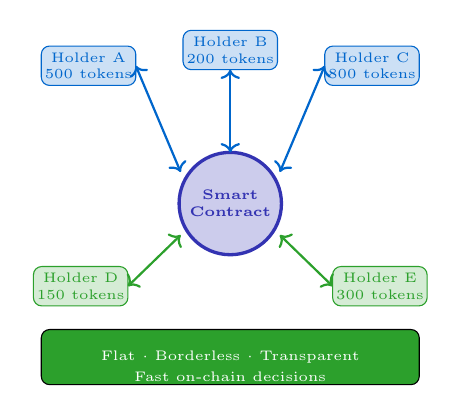
\begin{tikzpicture}
      % Smart contract center
      \draw[fill=mlpurple!25, draw=mlpurple, very thick] (2.5,2.8) circle (0.65);
      \node[font=\tiny\bfseries, mlpurple, align=center] at (2.5,2.8) {Smart\\Contract};
      % Token holder nodes
      \draw[fill=mlblue!20, draw=mlblue, rounded corners=3pt] (0.1,4.3) rectangle (1.3,4.8);
      \node[font=\tiny, mlblue, align=center] at (0.7,4.55) {Holder A\\500 tokens};
      \draw[fill=mlblue!20, draw=mlblue, rounded corners=3pt] (1.9,4.5) rectangle (3.1,5.0);
      \node[font=\tiny, mlblue, align=center] at (2.5,4.75) {Holder B\\200 tokens};
      \draw[fill=mlblue!20, draw=mlblue, rounded corners=3pt] (3.7,4.3) rectangle (4.9,4.8);
      \node[font=\tiny, mlblue, align=center] at (4.3,4.55) {Holder C\\800 tokens};
      \draw[fill=mlgreen!20, draw=mlgreen, rounded corners=3pt] (0.0,1.5) rectangle (1.2,2.0);
      \node[font=\tiny, mlgreen, align=center] at (0.6,1.75) {Holder D\\150 tokens};
      \draw[fill=mlgreen!20, draw=mlgreen, rounded corners=3pt] (3.8,1.5) rectangle (5.0,2.0);
      \node[font=\tiny, mlgreen, align=center] at (4.4,1.75) {Holder E\\300 tokens};
      % Lines from holders to center
      \draw[<->, thick, mlblue] (1.3,4.55) -- (1.87,3.2);
      \draw[<->, thick, mlblue] (2.5,4.5) -- (2.5,3.45);
      \draw[<->, thick, mlblue] (3.7,4.55) -- (3.13,3.2);
      \draw[<->, thick, mlgreen] (1.2,1.75) -- (1.87,2.4);
      \draw[<->, thick, mlgreen] (3.8,1.75) -- (3.13,2.4);
      % DAO label
      \draw[fill=mlgreen, rounded corners=3pt] (0.1,0.5) rectangle (4.9,1.2);
      \node[font=\tiny, white, align=center] at (2.5,0.85) {Flat $\cdot$ Borderless $\cdot$ Transparent};
      \node[font=\tiny, white, align=center] at (2.5,0.6) {Fast on-chain decisions};
    \end{tikzpicture}
  \end{column}
\end{columns}

\vspace{0.1cm}
\begin{center}

\begin{tikzpicture}
  \draw[fill=mlpurple!10, draw=mlpurple, rounded corners=4pt] (0,0) rectangle (12.5,0.7);
  \node[font=\tiny\bfseries, mlpurple] at (2.1,0.5) {Hierarchy vs Flat};
  \node[font=\tiny, mlgray] at (2.1,0.22) {CEO decides alone};
  \node[font=\tiny\bfseries, mlpurple] at (5.0,0.5) {Borders vs Borderless};
  \node[font=\tiny, mlgray] at (5.0,0.22) {Global participation};
  \node[font=\tiny\bfseries, mlpurple] at (8.0,0.5) {Closed vs Transparent};
  \node[font=\tiny, mlgray] at (8.0,0.22) {All votes on-chain};
  \node[font=\tiny\bfseries, mlpurple] at (11.0,0.5) {Slow vs Automated};
  \node[font=\tiny, mlgray] at (11.0,0.22) {Code executes instantly};
\end{tikzpicture}
\end{center}

\bottomnote{Traditional organizations rely on hierarchical authority; DAOs replace the hierarchy with transparent, code-enforced rules and token-weighted democratic voting.}
\end{frame}

% Frame 4: How Voting Works
\begin{frame}{How Voting Works in a DAO}
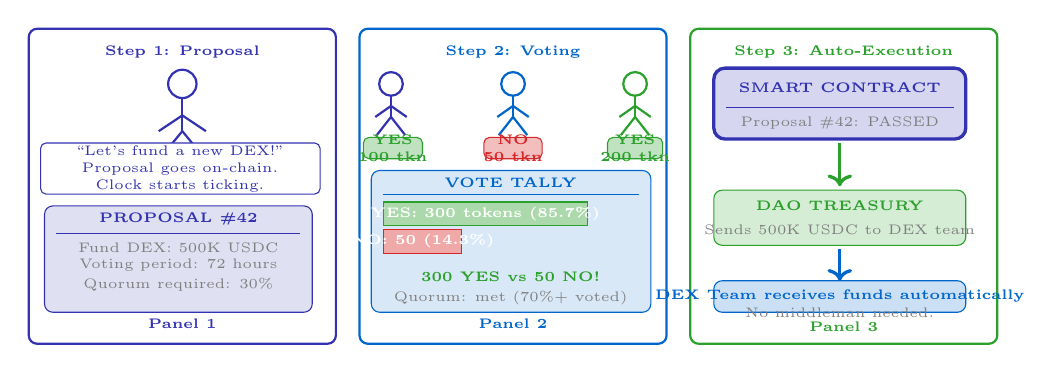
\begin{tikzpicture}
  % Panel borders
  \draw[thick, mlpurple, rounded corners=3pt] (0.1,0.2) rectangle (4.0,4.2);
  \draw[thick, mlblue,   rounded corners=3pt] (4.3,0.2) rectangle (8.2,4.2);
  \draw[thick, mlgreen,  rounded corners=3pt] (8.5,0.2) rectangle (12.4,4.2);

  % --- Panel 1: Proposal submitted ---
  \node[font=\tiny\bfseries, mlpurple] at (2.05,3.9) {Step 1: Proposal};
  % Person submitting
  \draw[mlpurple,thick] (2.05,3.5) circle (0.18);
  \draw[mlpurple,thick] (2.05,3.32) -- (2.05,2.9);
  \draw[mlpurple,thick] (2.05,3.1) -- (1.75,2.9);
  \draw[mlpurple,thick] (2.05,3.1) -- (2.35,2.9);
  \draw[mlpurple,thick] (2.05,2.9) -- (1.82,2.62);
  \draw[mlpurple,thick] (2.05,2.9) -- (2.28,2.62);
  % Speech bubble
  \draw[fill=white, draw=mlpurple, rounded corners=2pt] (0.25,2.1) rectangle (3.8,2.75);
  \node[font=\tiny, mlpurple, align=center] at (2.02,2.42) {``Let's fund a new DEX!''\\Proposal goes on-chain.\\Clock starts ticking.};
  % Proposal box
  \draw[fill=mlpurple!15, draw=mlpurple, rounded corners=3pt] (0.3,0.6) rectangle (3.7,1.95);
  \node[font=\tiny\bfseries, mlpurple, align=center] at (2.0,1.78) {PROPOSAL \#42};
  \draw[mlpurple, thin] (0.45,1.6) -- (3.55,1.6);
  \node[font=\tiny, mlgray, align=center] at (2.0,1.42) {Fund DEX: 500K USDC};
  \node[font=\tiny, mlgray, align=center] at (2.0,1.2) {Voting period: 72 hours};
  \node[font=\tiny, mlgray, align=center] at (2.0,0.95) {Quorum required: 30\%};
  \node[font=\tiny\bfseries, mlpurple] at (2.05,0.45) {Panel 1};

  % --- Panel 2: Token holders vote ---
  \node[font=\tiny\bfseries, mlblue] at (6.25,3.9) {Step 2: Voting};
  % Alice votes YES
  \draw[mlpurple,thick] (4.7,3.5) circle (0.15);
  \draw[mlpurple,thick] (4.7,3.35) -- (4.7,3.08);
  \draw[mlpurple,thick] (4.7,3.22) -- (4.5,3.08);
  \draw[mlpurple,thick] (4.7,3.22) -- (4.9,3.08);
  \draw[mlpurple,thick] (4.7,3.08) -- (4.52,2.85);
  \draw[mlpurple,thick] (4.7,3.08) -- (4.88,2.85);
  \draw[fill=mlgreen!30, draw=mlgreen, rounded corners=2pt] (4.35,2.55) rectangle (5.1,2.82);
  \node[font=\tiny\bfseries, mlgreen, align=center] at (4.72,2.68) {YES\\100 tkn};
  % Bob votes NO
  \draw[mlblue,thick] (6.25,3.5) circle (0.15);
  \draw[mlblue,thick] (6.25,3.35) -- (6.25,3.08);
  \draw[mlblue,thick] (6.25,3.22) -- (6.05,3.08);
  \draw[mlblue,thick] (6.25,3.22) -- (6.45,3.08);
  \draw[mlblue,thick] (6.25,3.08) -- (6.07,2.85);
  \draw[mlblue,thick] (6.25,3.08) -- (6.43,2.85);
  \draw[fill=mlred!30, draw=mlred, rounded corners=2pt] (5.88,2.55) rectangle (6.62,2.82);
  \node[font=\tiny\bfseries, mlred, align=center] at (6.25,2.68) {NO\\50 tkn};
  % Charlie votes YES
  \draw[mlgreen,thick] (7.8,3.5) circle (0.15);
  \draw[mlgreen,thick] (7.8,3.35) -- (7.8,3.08);
  \draw[mlgreen,thick] (7.8,3.22) -- (7.6,3.08);
  \draw[mlgreen,thick] (7.8,3.22) -- (8.0,3.08);
  \draw[mlgreen,thick] (7.8,3.08) -- (7.62,2.85);
  \draw[mlgreen,thick] (7.8,3.08) -- (7.98,2.85);
  \draw[fill=mlgreen!30, draw=mlgreen, rounded corners=2pt] (7.45,2.55) rectangle (8.15,2.82);
  \node[font=\tiny\bfseries, mlgreen, align=center] at (7.8,2.68) {YES\\200 tkn};
  % Vote tally
  \draw[fill=mlblue!15, draw=mlblue, rounded corners=3pt] (4.45,0.6) rectangle (8.0,2.4);
  \node[font=\tiny\bfseries, mlblue, align=center] at (6.22,2.25) {VOTE TALLY};
  \draw[mlblue, thin] (4.6,2.1) -- (7.85,2.1);
  \draw[fill=mlgreen!40, draw=mlgreen] (4.6,1.7) rectangle (7.2,2.0);
  \node[font=\tiny\bfseries, white, align=center] at (5.9,1.85) {YES: 300 tokens (85.7\%)};
  \draw[fill=mlred!40, draw=mlred] (4.6,1.35) rectangle (5.6,1.65);
  \node[font=\tiny\bfseries, white, align=center] at (5.1,1.5) {NO: 50 (14.3\%)};
  \node[font=\tiny\bfseries, mlgreen, align=center] at (6.22,1.05) {300 YES vs 50 NO!};
  \node[font=\tiny, mlgray, align=center] at (6.22,0.78) {Quorum: met (70\%+ voted)};
  \node[font=\tiny\bfseries, mlblue] at (6.25,0.45) {Panel 2};

  % --- Panel 3: Proposal passes, auto-executes ---
  \node[font=\tiny\bfseries, mlgreen] at (10.45,3.9) {Step 3: Auto-Execution};
  % Smart contract
  \draw[fill=mlpurple!20, draw=mlpurple, very thick, rounded corners=4pt] (8.8,2.8) rectangle (12.0,3.7);
  \node[font=\tiny\bfseries, mlpurple, align=center] at (10.4,3.45) {SMART CONTRACT};
  \draw[mlpurple, thin] (8.95,3.2) -- (11.85,3.2);
  \node[font=\tiny, mlgray, align=center] at (10.4,3.0) {Proposal \#42: PASSED};
  % Arrow down to treasury
  \draw[->, very thick, mlgreen] (10.4,2.75) -- (10.4,2.2);
  % Treasury box
  \draw[fill=mlgreen!20, draw=mlgreen, rounded corners=3pt] (8.8,1.45) rectangle (12.0,2.15);
  \node[font=\tiny\bfseries, mlgreen, align=center] at (10.4,1.95) {DAO TREASURY};
  \node[font=\tiny, mlgray, align=center] at (10.4,1.65) {Sends 500K USDC to DEX team};
  % Arrow to DEX
  \draw[->, very thick, mlblue] (10.4,1.4) -- (10.4,1.0);
  \draw[fill=mlblue!20, draw=mlblue, rounded corners=3pt] (8.8,0.6) rectangle (12.0,1.0);
  \node[font=\tiny\bfseries, mlblue, align=center] at (10.4,0.8) {DEX Team receives funds automatically};
  \node[font=\tiny, mlgray, align=center] at (10.4,0.6) {No middleman needed.};
  \node[font=\tiny\bfseries, mlgreen] at (10.45,0.42) {Panel 3};
\end{tikzpicture}

\bottomnote{DAO governance: anyone can submit a proposal; token holders vote (token-weighted); smart contracts automatically execute approved proposals -- no human intermediary.}
\end{frame}

% Frame 5: Types of DAOs
\begin{frame}{Types of DAOs}
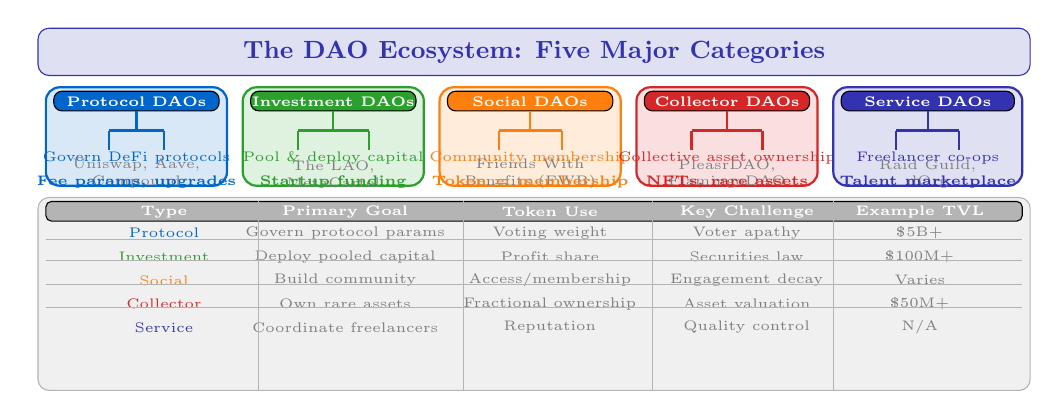
\begin{tikzpicture}
  % Header
  \draw[fill=mlpurple!15, draw=mlpurple, rounded corners=4pt] (0.0,4.3) rectangle (12.6,4.9);
  \node[font=\small\bfseries, mlpurple, align=center] at (6.3,4.6) {The DAO Ecosystem: Five Major Categories};

  % Box 1: Protocol DAOs
  \draw[fill=mlblue!15, draw=mlblue, rounded corners=5pt, thick] (0.1,2.9) rectangle (2.4,4.15);
  \draw[fill=mlblue, rounded corners=3pt] (0.2,3.85) rectangle (2.3,4.1);
  \node[font=\tiny\bfseries, white, align=center] at (1.25,3.97) {Protocol DAOs};
  \draw[mlblue, thick] (1.25,3.85) -- (1.25,3.6);
  \draw[mlblue, thick] (0.9,3.6) -- (1.6,3.6);
  \draw[mlblue, thick] (0.9,3.6) -- (0.9,3.35);
  \draw[mlblue, thick] (1.6,3.6) -- (1.6,3.35);
  \node[font=\tiny, mlblue, align=center] at (1.25,3.25) {Govern DeFi protocols};
  \node[font=\tiny, mlgray, align=center] at (1.25,3.05) {Uniswap, Aave,\\Compound};
  \node[font=\tiny\bfseries, mlblue, align=center] at (1.25,2.95) {Fee params, upgrades};

  % Box 2: Investment DAOs
  \draw[fill=mlgreen!15, draw=mlgreen, rounded corners=5pt, thick] (2.6,2.9) rectangle (4.9,4.15);
  \draw[fill=mlgreen, rounded corners=3pt] (2.7,3.85) rectangle (4.8,4.1);
  \node[font=\tiny\bfseries, white, align=center] at (3.75,3.97) {Investment DAOs};
  \draw[mlgreen, thick] (3.75,3.85) -- (3.75,3.6);
  \draw[mlgreen, thick] (3.3,3.6) -- (4.2,3.6);
  \draw[mlgreen, thick] (3.3,3.6) -- (3.3,3.35);
  \draw[mlgreen, thick] (4.2,3.6) -- (4.2,3.35);
  \node[font=\tiny, mlgreen, align=center] at (3.75,3.25) {Pool \& deploy capital};
  \node[font=\tiny, mlgray, align=center] at (3.75,3.05) {The LAO,\\MetaCartel};
  \node[font=\tiny\bfseries, mlgreen, align=center] at (3.75,2.95) {Startup funding};

  % Box 3: Social DAOs
  \draw[fill=mlorange!15, draw=mlorange, rounded corners=5pt, thick] (5.1,2.9) rectangle (7.4,4.15);
  \draw[fill=mlorange, rounded corners=3pt] (5.2,3.85) rectangle (7.3,4.1);
  \node[font=\tiny\bfseries, white, align=center] at (6.25,3.97) {Social DAOs};
  \draw[mlorange, thick] (6.25,3.85) -- (6.25,3.6);
  \draw[mlorange, thick] (5.85,3.6) -- (6.65,3.6);
  \draw[mlorange, thick] (5.85,3.6) -- (5.85,3.35);
  \draw[mlorange, thick] (6.65,3.6) -- (6.65,3.35);
  \node[font=\tiny, mlorange, align=center] at (6.25,3.25) {Community membership};
  \node[font=\tiny, mlgray, align=center] at (6.25,3.05) {Friends With\\Benefits (FWB)};
  \node[font=\tiny\bfseries, mlorange, align=center] at (6.25,2.95) {Token = membership};

  % Box 4: Collector DAOs
  \draw[fill=mlred!15, draw=mlred, rounded corners=5pt, thick] (7.6,2.9) rectangle (9.9,4.15);
  \draw[fill=mlred, rounded corners=3pt] (7.7,3.85) rectangle (9.8,4.1);
  \node[font=\tiny\bfseries, white, align=center] at (8.75,3.97) {Collector DAOs};
  \draw[mlred, thick] (8.75,3.85) -- (8.75,3.6);
  \draw[mlred, thick] (8.3,3.6) -- (9.2,3.6);
  \draw[mlred, thick] (8.3,3.6) -- (8.3,3.35);
  \draw[mlred, thick] (9.2,3.6) -- (9.2,3.35);
  \node[font=\tiny, mlred, align=center] at (8.75,3.25) {Collective asset ownership};
  \node[font=\tiny, mlgray, align=center] at (8.75,3.05) {PleasrDAO,\\FlamingoDAO};
  \node[font=\tiny\bfseries, mlred, align=center] at (8.75,2.95) {NFTs, rare assets};

  % Box 5: Service DAOs
  \draw[fill=mlpurple!15, draw=mlpurple, rounded corners=5pt, thick] (10.1,2.9) rectangle (12.5,4.15);
  \draw[fill=mlpurple, rounded corners=3pt] (10.2,3.85) rectangle (12.4,4.1);
  \node[font=\tiny\bfseries, white, align=center] at (11.3,3.97) {Service DAOs};
  \draw[mlpurple, thick] (11.3,3.85) -- (11.3,3.6);
  \draw[mlpurple, thick] (10.9,3.6) -- (11.7,3.6);
  \draw[mlpurple, thick] (10.9,3.6) -- (10.9,3.35);
  \draw[mlpurple, thick] (11.7,3.6) -- (11.7,3.35);
  \node[font=\tiny, mlpurple, align=center] at (11.3,3.25) {Freelancer co-ops};
  \node[font=\tiny, mlgray, align=center] at (11.3,3.05) {Raid Guild,\\dOrg};
  \node[font=\tiny\bfseries, mlpurple, align=center] at (11.3,2.95) {Talent marketplace};

  % Comparison table at bottom
  \draw[fill=lightgray, draw=midgray, rounded corners=4pt] (0.0,0.3) rectangle (12.6,2.75);
  % Header row
  \draw[fill=midgray, rounded corners=2pt] (0.1,2.45) rectangle (12.5,2.7);
  \node[font=\tiny\bfseries, white] at (1.6,2.57) {Type};
  \node[font=\tiny\bfseries, white] at (3.9,2.57) {Primary Goal};
  \node[font=\tiny\bfseries, white] at (6.5,2.57) {Token Use};
  \node[font=\tiny\bfseries, white] at (9.0,2.57) {Key Challenge};
  \node[font=\tiny\bfseries, white] at (11.2,2.57) {Example TVL};
  % Row 1
  \node[font=\tiny, mlblue]  at (1.6,2.3) {Protocol};
  \node[font=\tiny, mlgray]  at (3.9,2.3) {Govern protocol params};
  \node[font=\tiny, mlgray]  at (6.5,2.3) {Voting weight};
  \node[font=\tiny, mlgray]  at (9.0,2.3) {Voter apathy};
  \node[font=\tiny, mlgray]  at (11.2,2.3) {\$5B+};
  % Row 2
  \node[font=\tiny, mlgreen] at (1.6,2.0) {Investment};
  \node[font=\tiny, mlgray]  at (3.9,2.0) {Deploy pooled capital};
  \node[font=\tiny, mlgray]  at (6.5,2.0) {Profit share};
  \node[font=\tiny, mlgray]  at (9.0,2.0) {Securities law};
  \node[font=\tiny, mlgray]  at (11.2,2.0) {\$100M+};
  % Row 3
  \node[font=\tiny, mlorange] at (1.6,1.7) {Social};
  \node[font=\tiny, mlgray]   at (3.9,1.7) {Build community};
  \node[font=\tiny, mlgray]   at (6.5,1.7) {Access/membership};
  \node[font=\tiny, mlgray]   at (9.0,1.7) {Engagement decay};
  \node[font=\tiny, mlgray]   at (11.2,1.7) {Varies};
  % Row 4
  \node[font=\tiny, mlred]  at (1.6,1.4) {Collector};
  \node[font=\tiny, mlgray] at (3.9,1.4) {Own rare assets};
  \node[font=\tiny, mlgray] at (6.5,1.4) {Fractional ownership};
  \node[font=\tiny, mlgray] at (9.0,1.4) {Asset valuation};
  \node[font=\tiny, mlgray] at (11.2,1.4) {\$50M+};
  % Row 5
  \node[font=\tiny, mlpurple] at (1.6,1.1) {Service};
  \node[font=\tiny, mlgray]   at (3.9,1.1) {Coordinate freelancers};
  \node[font=\tiny, mlgray]   at (6.5,1.1) {Reputation};
  \node[font=\tiny, mlgray]   at (9.0,1.1) {Quality control};
  \node[font=\tiny, mlgray]   at (11.2,1.1) {N/A};
  % Dividers
  \draw[midgray, thin] (0.1,1.95) -- (12.5,1.95);
  \draw[midgray, thin] (0.1,2.22) -- (12.5,2.22);
  \draw[midgray, thin] (0.1,1.65) -- (12.5,1.65);
  \draw[midgray, thin] (0.1,1.35) -- (12.5,1.35);
  \draw[midgray, thin] (2.8,0.3)  -- (2.8,2.7);
  \draw[midgray, thin] (5.4,0.3)  -- (5.4,2.7);
  \draw[midgray, thin] (7.8,0.3)  -- (7.8,2.7);
  \draw[midgray, thin] (10.1,0.3) -- (10.1,2.7);
\end{tikzpicture}

\bottomnote{DAOs are not one-size-fits-all. Protocol DAOs govern DeFi, investment DAOs pool capital, social DAOs build community, collector DAOs own NFTs, service DAOs coordinate work.}
\end{frame}

% Frame 6: The DAO Hack
\begin{frame}{The DAO Hack of 2016: A Defining Moment}
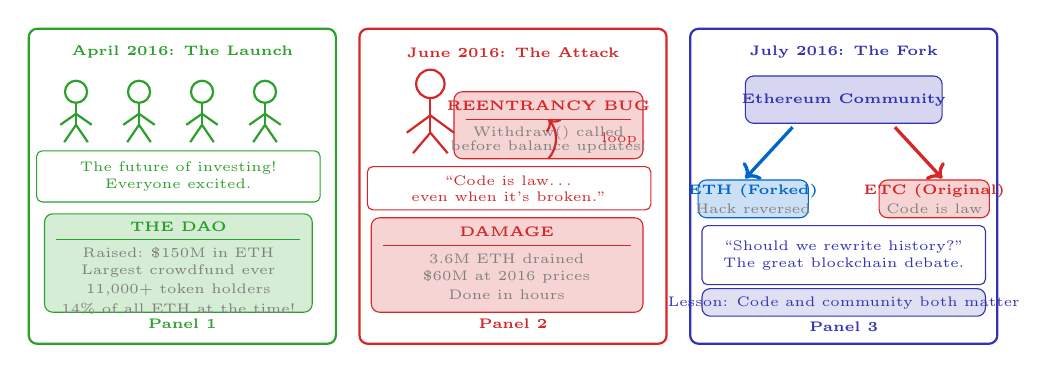
\begin{tikzpicture}
  % Panel borders
  \draw[thick, mlgreen,  rounded corners=3pt] (0.1,0.2) rectangle (4.0,4.2);
  \draw[thick, mlred,    rounded corners=3pt] (4.3,0.2) rectangle (8.2,4.2);
  \draw[thick, mlpurple, rounded corners=3pt] (8.5,0.2) rectangle (12.4,4.2);

  % --- Panel 1: The DAO launches ---
  \node[font=\tiny\bfseries, mlgreen] at (2.05,3.9) {April 2016: The Launch};
  % Crowd of stick figures
  \draw[mlgreen,thick] (0.7,3.4) circle (0.14);
  \draw[mlgreen,thick] (0.7,3.26) -- (0.7,2.98);
  \draw[mlgreen,thick] (0.7,3.12) -- (0.5,2.98);
  \draw[mlgreen,thick] (0.7,3.12) -- (0.9,2.98);
  \draw[mlgreen,thick] (0.7,2.98) -- (0.55,2.76);
  \draw[mlgreen,thick] (0.7,2.98) -- (0.85,2.76);
  \draw[mlgreen,thick] (1.5,3.4) circle (0.14);
  \draw[mlgreen,thick] (1.5,3.26) -- (1.5,2.98);
  \draw[mlgreen,thick] (1.5,3.12) -- (1.3,2.98);
  \draw[mlgreen,thick] (1.5,3.12) -- (1.7,2.98);
  \draw[mlgreen,thick] (1.5,2.98) -- (1.35,2.76);
  \draw[mlgreen,thick] (1.5,2.98) -- (1.65,2.76);
  \draw[mlgreen,thick] (2.3,3.4) circle (0.14);
  \draw[mlgreen,thick] (2.3,3.26) -- (2.3,2.98);
  \draw[mlgreen,thick] (2.3,3.12) -- (2.1,2.98);
  \draw[mlgreen,thick] (2.3,3.12) -- (2.5,2.98);
  \draw[mlgreen,thick] (2.3,2.98) -- (2.15,2.76);
  \draw[mlgreen,thick] (2.3,2.98) -- (2.45,2.76);
  \draw[mlgreen,thick] (3.1,3.4) circle (0.14);
  \draw[mlgreen,thick] (3.1,3.26) -- (3.1,2.98);
  \draw[mlgreen,thick] (3.1,3.12) -- (2.9,2.98);
  \draw[mlgreen,thick] (3.1,3.12) -- (3.3,2.98);
  \draw[mlgreen,thick] (3.1,2.98) -- (2.95,2.76);
  \draw[mlgreen,thick] (3.1,2.98) -- (3.25,2.76);
  % Speech bubble
  \draw[fill=white, draw=mlgreen, rounded corners=2pt] (0.2,2.0) rectangle (3.8,2.65);
  \node[font=\tiny, mlgreen, align=center] at (2.0,2.32) {The future of investing!\\Everyone excited.};
  % Stats box
  \draw[fill=mlgreen!20, draw=mlgreen, rounded corners=3pt] (0.3,0.6) rectangle (3.7,1.85);
  \node[font=\tiny\bfseries, mlgreen, align=center] at (2.0,1.68) {THE DAO};
  \draw[mlgreen, thin] (0.45,1.52) -- (3.55,1.52);
  \node[font=\tiny, mlgray, align=center] at (2.0,1.35) {Raised: \$150M in ETH};
  \node[font=\tiny, mlgray, align=center] at (2.0,1.12) {Largest crowdfund ever};
  \node[font=\tiny, mlgray, align=center] at (2.0,0.88) {11,000+ token holders};
  \node[font=\tiny, mlgray, align=center] at (2.0,0.65) {14\% of all ETH at the time!};
  \node[font=\tiny\bfseries, mlgreen] at (2.05,0.45) {Panel 1};

  % --- Panel 2: The hack ---
  \node[font=\tiny\bfseries, mlred] at (6.25,3.9) {June 2016: The Attack};
  % Hacker figure (sinister)
  \draw[mlred,thick] (5.2,3.5) circle (0.18);
  \draw[mlred,thick] (5.2,3.32) -- (5.2,2.88);
  \draw[mlred,thick] (5.2,3.1) -- (4.9,2.88);
  \draw[mlred,thick] (5.2,3.1) -- (5.5,2.88);
  \draw[mlred,thick] (5.2,2.88) -- (4.98,2.62);
  \draw[mlred,thick] (5.2,2.88) -- (5.42,2.62);
  % Bug icon
  \draw[fill=mlred!20, draw=mlred, rounded corners=3pt] (5.5,2.55) rectangle (7.9,3.4);
  \node[font=\tiny\bfseries, mlred, align=center] at (6.7,3.22) {REENTRANCY BUG};
  \draw[mlred, thin] (5.65,3.05) -- (7.75,3.05);
  \node[font=\tiny, mlgray, align=center] at (6.7,2.88) {Withdraw() called};
  \node[font=\tiny, mlgray, align=center] at (6.7,2.7) {before balance updates!};
  % Arrow loop showing reentrancy
  \draw[->, thick, mlred] (6.7,2.55) to[bend right=40] (6.7,3.05);
  \node[font=\tiny, mlred] at (7.6,2.8) {loop};
  % Speech bubble
  \draw[fill=white, draw=mlred, rounded corners=2pt] (4.4,1.9) rectangle (8.0,2.45);
  \node[font=\tiny, mlred, align=center] at (6.2,2.17) {``Code is law\ldots\\even when it's broken.''};
  % Damage box
  \draw[fill=mlred!20, draw=mlred, rounded corners=3pt] (4.45,0.6) rectangle (7.9,1.8);
  \node[font=\tiny\bfseries, mlred, align=center] at (6.17,1.62) {DAMAGE};
  \draw[mlred, thin] (4.6,1.45) -- (7.75,1.45);
  \node[font=\tiny, mlgray, align=center] at (6.17,1.28) {3.6M ETH drained};
  \node[font=\tiny, mlgray, align=center] at (6.17,1.05) {\$60M at 2016 prices};
  \node[font=\tiny, mlgray, align=center] at (6.17,0.82) {Done in hours};
  \node[font=\tiny\bfseries, mlred] at (6.25,0.45) {Panel 2};

  % --- Panel 3: The fork ---
  \node[font=\tiny\bfseries, mlpurple] at (10.45,3.9) {July 2016: The Fork};
  % Split diagram
  \draw[fill=mlpurple!20, draw=mlpurple, rounded corners=3pt] (9.2,3.0) rectangle (11.7,3.6);
  \node[font=\tiny\bfseries, mlpurple, align=center] at (10.45,3.3) {Ethereum Community};
  % Fork arrow left (ETH)
  \draw[->, very thick, mlblue] (9.8,2.95) -- (9.2,2.3);
  \draw[fill=mlblue!20, draw=mlblue, rounded corners=3pt] (8.6,1.8) rectangle (10.0,2.28);
  \node[font=\tiny\bfseries, mlblue, align=center] at (9.3,2.14) {ETH (Forked)};
  \node[font=\tiny, mlgray, align=center] at (9.3,1.92) {Hack reversed};
  % Fork arrow right (ETC)
  \draw[->, very thick, mlred] (11.1,2.95) -- (11.7,2.3);
  \draw[fill=mlred!20, draw=mlred, rounded corners=3pt] (10.9,1.8) rectangle (12.3,2.28);
  \node[font=\tiny\bfseries, mlred, align=center] at (11.6,2.14) {ETC (Original)};
  \node[font=\tiny, mlgray, align=center] at (11.6,1.92) {Code is law};
  % Debate bubble
  \draw[fill=white, draw=mlpurple, rounded corners=2pt] (8.65,0.95) rectangle (12.25,1.7);
  \node[font=\tiny, mlpurple, align=center] at (10.45,1.32) {``Should we rewrite history?''\\The great blockchain debate.};
  % Lesson box
  \draw[fill=mlpurple!15, draw=mlpurple, rounded corners=3pt] (8.65,0.55) rectangle (12.25,0.9);
  \node[font=\tiny, mlpurple, align=center] at (10.45,0.72) {Lesson: Code and community both matter};
  \node[font=\tiny\bfseries, mlpurple] at (10.45,0.42) {Panel 3};
\end{tikzpicture}

\bottomnote{The 2016 DAO hack drained \$60M via a reentrancy vulnerability. Ethereum hard-forked to reverse the theft, splitting the chain into ETH and ETC -- a pivotal moment in blockchain history.}
\end{frame}

% Frame 7: Treasury Management
\begin{frame}{DAO Treasury Management}
\begin{columns}[c]
  \begin{column}{0.58\textwidth}
    \centering
    {\small\bfseries\color{mlpurple} Multi-Sig Treasury Architecture}\\[0.15cm]
    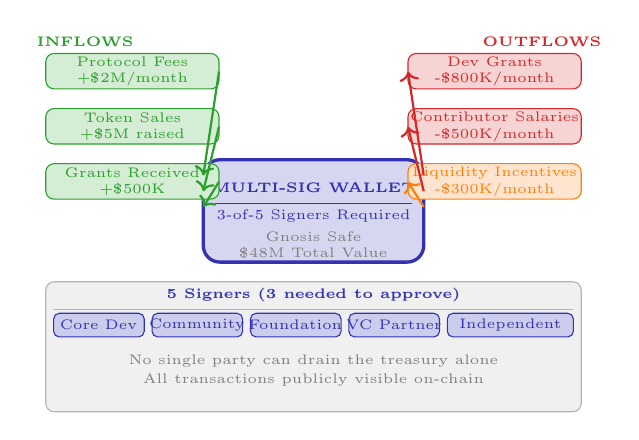
\begin{tikzpicture}
      % Central multi-sig wallet
      \draw[fill=mlpurple!20, draw=mlpurple, very thick, rounded corners=6pt] (2.0,2.0) rectangle (4.8,3.3);
      \node[font=\tiny\bfseries, mlpurple, align=center] at (3.4,2.95) {MULTI-SIG WALLET};
      \draw[mlpurple, thin] (2.15,2.75) -- (4.65,2.75);
      \node[font=\tiny, mlpurple, align=center] at (3.4,2.58) {3-of-5 Signers Required};
      \node[font=\tiny, mlgray, align=center] at (3.4,2.32) {Gnosis Safe};
      \node[font=\tiny, mlgray, align=center] at (3.4,2.12) {\$48M Total Value};

      % Inflow sources (left side)
      \node[font=\tiny\bfseries, mlgreen] at (0.5,4.8) {INFLOWS};
      \draw[fill=mlgreen!20, draw=mlgreen, rounded corners=3pt] (0.0,4.2) rectangle (2.2,4.65);
      \node[font=\tiny, mlgreen, align=center] at (1.1,4.42) {Protocol Fees\\+\$2M/month};
      \draw[fill=mlgreen!20, draw=mlgreen, rounded corners=3pt] (0.0,3.5) rectangle (2.2,3.95);
      \node[font=\tiny, mlgreen, align=center] at (1.1,3.72) {Token Sales\\+\$5M raised};
      \draw[fill=mlgreen!20, draw=mlgreen, rounded corners=3pt] (0.0,2.8) rectangle (2.2,3.25);
      \node[font=\tiny, mlgreen, align=center] at (1.1,3.02) {Grants Received\\+\$500K};
      % Arrows from inflows to wallet
      \draw[->, thick, mlgreen] (2.2,4.42) -- (2.0,3.1);
      \draw[->, thick, mlgreen] (2.2,3.72) -- (2.0,2.9);
      \draw[->, thick, mlgreen] (2.2,3.02) -- (2.0,2.7);

      % Outflow uses (right side)
      \node[font=\tiny\bfseries, mlred] at (6.3,4.8) {OUTFLOWS};
      \draw[fill=mlred!20, draw=mlred, rounded corners=3pt] (4.6,4.2) rectangle (6.8,4.65);
      \node[font=\tiny, mlred, align=center] at (5.7,4.42) {Dev Grants\\-\$800K/month};
      \draw[fill=mlred!20, draw=mlred, rounded corners=3pt] (4.6,3.5) rectangle (6.8,3.95);
      \node[font=\tiny, mlred, align=center] at (5.7,3.72) {Contributor Salaries\\-\$500K/month};
      \draw[fill=mlorange!20, draw=mlorange, rounded corners=3pt] (4.6,2.8) rectangle (6.8,3.25);
      \node[font=\tiny, mlorange, align=center] at (5.7,3.02) {Liquidity Incentives\\-\$300K/month};
      % Arrows from wallet to outflows
      \draw[->, thick, mlred] (4.8,3.1) -- (4.6,4.42);
      \draw[->, thick, mlred] (4.8,2.9) -- (4.6,3.72);
      \draw[->, thick, mlorange] (4.8,2.7) -- (4.6,3.02);

      % Signer list at bottom
      \draw[fill=lightgray, draw=midgray, rounded corners=3pt] (0.0,0.1) rectangle (6.8,1.75);
      \node[font=\tiny\bfseries, mlpurple, align=center] at (3.4,1.58) {5 Signers (3 needed to approve)};
      \draw[midgray, thin] (0.1,1.4) -- (6.7,1.4);
      \draw[fill=mlpurple!25, draw=mlpurple, rounded corners=2pt] (0.1,1.05) rectangle (1.25,1.35);
      \node[font=\tiny, mlpurple, align=center] at (0.67,1.2) {Core Dev};
      \draw[fill=mlpurple!25, draw=mlpurple, rounded corners=2pt] (1.35,1.05) rectangle (2.5,1.35);
      \node[font=\tiny, mlpurple, align=center] at (1.92,1.2) {Community};
      \draw[fill=mlpurple!25, draw=mlpurple, rounded corners=2pt] (2.6,1.05) rectangle (3.75,1.35);
      \node[font=\tiny, mlpurple, align=center] at (3.17,1.2) {Foundation};
      \draw[fill=mlpurple!25, draw=mlpurple, rounded corners=2pt] (3.85,1.05) rectangle (5.0,1.35);
      \node[font=\tiny, mlpurple, align=center] at (4.42,1.2) {VC Partner};
      \draw[fill=mlpurple!25, draw=mlpurple, rounded corners=2pt] (5.1,1.05) rectangle (6.7,1.35);
      \node[font=\tiny, mlpurple, align=center] at (5.9,1.2) {Independent};
      \node[font=\tiny, mlgray, align=center] at (3.4,0.75) {No single party can drain the treasury alone};
      \node[font=\tiny, mlgray, align=center] at (3.4,0.5) {All transactions publicly visible on-chain};
    \end{tikzpicture}
  \end{column}

  \begin{column}{0.40\textwidth}
    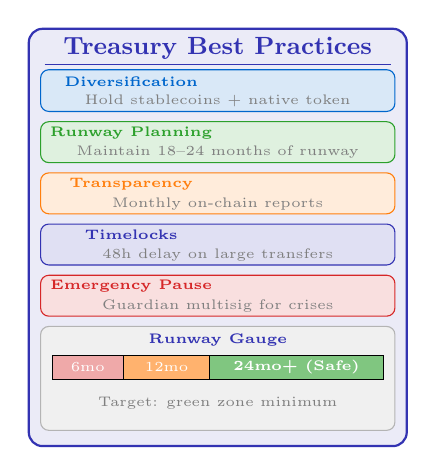
\begin{tikzpicture}
      % Best practices
      \draw[fill=mlpurple!10, draw=mlpurple, rounded corners=5pt, thick] (0,0) rectangle (4.8,5.3);
      \node[font=\small\bfseries, mlpurple, align=center] at (2.4,5.05) {Treasury Best Practices};
      \draw[mlpurple, thin] (0.2,4.85) -- (4.6,4.85);

      \draw[fill=mlblue!15, draw=mlblue, rounded corners=3pt] (0.15,4.25) rectangle (4.65,4.78);
      \node[font=\tiny\bfseries, mlblue, align=left] at (1.3,4.63) {Diversification};
      \node[font=\tiny, mlgray, align=left] at (2.4,4.38) {Hold stablecoins + native token};

      \draw[fill=mlgreen!15, draw=mlgreen, rounded corners=3pt] (0.15,3.6) rectangle (4.65,4.12);
      \node[font=\tiny\bfseries, mlgreen, align=left] at (1.3,3.98) {Runway Planning};
      \node[font=\tiny, mlgray, align=left] at (2.4,3.73) {Maintain 18--24 months of runway};

      \draw[fill=mlorange!15, draw=mlorange, rounded corners=3pt] (0.15,2.95) rectangle (4.65,3.47);
      \node[font=\tiny\bfseries, mlorange, align=left] at (1.3,3.33) {Transparency};
      \node[font=\tiny, mlgray, align=left] at (2.4,3.08) {Monthly on-chain reports};

      \draw[fill=mlpurple!15, draw=mlpurple, rounded corners=3pt] (0.15,2.3) rectangle (4.65,2.82);
      \node[font=\tiny\bfseries, mlpurple, align=left] at (1.3,2.68) {Timelocks};
      \node[font=\tiny, mlgray, align=left] at (2.4,2.43) {48h delay on large transfers};

      \draw[fill=mlred!15, draw=mlred, rounded corners=3pt] (0.15,1.65) rectangle (4.65,2.17);
      \node[font=\tiny\bfseries, mlred, align=left] at (1.3,2.03) {Emergency Pause};
      \node[font=\tiny, mlgray, align=left] at (2.4,1.78) {Guardian multisig for crises};

      % Runway gauge
      \draw[fill=lightgray, draw=midgray, rounded corners=3pt] (0.15,0.2) rectangle (4.65,1.52);
      \node[font=\tiny\bfseries, mlpurple, align=center] at (2.4,1.35) {Runway Gauge};
      \draw[fill=mlred!40]   (0.3,0.85) rectangle (1.2,1.15);
      \draw[fill=mlorange!60] (1.2,0.85) rectangle (2.3,1.15);
      \draw[fill=mlgreen!60] (2.3,0.85) rectangle (4.5,1.15);
      \node[font=\tiny, white, align=center] at (0.75,1.0) {6mo};
      \node[font=\tiny, white, align=center] at (1.75,1.0) {12mo};
      \node[font=\tiny\bfseries, white, align=center] at (3.4,1.0) {24mo+ (Safe)};
      \node[font=\tiny, mlgray, align=center] at (2.4,0.55) {Target: green zone minimum};
    \end{tikzpicture}
  \end{column}
\end{columns}

\bottomnote{DAO treasuries use multi-signature wallets (e.g., Gnosis Safe) requiring multiple approvers per transaction, providing security through distributed control and full on-chain transparency.}
\end{frame}

% Frame 8: Governance Attacks
\begin{frame}{Governance Attacks: Real Threats}
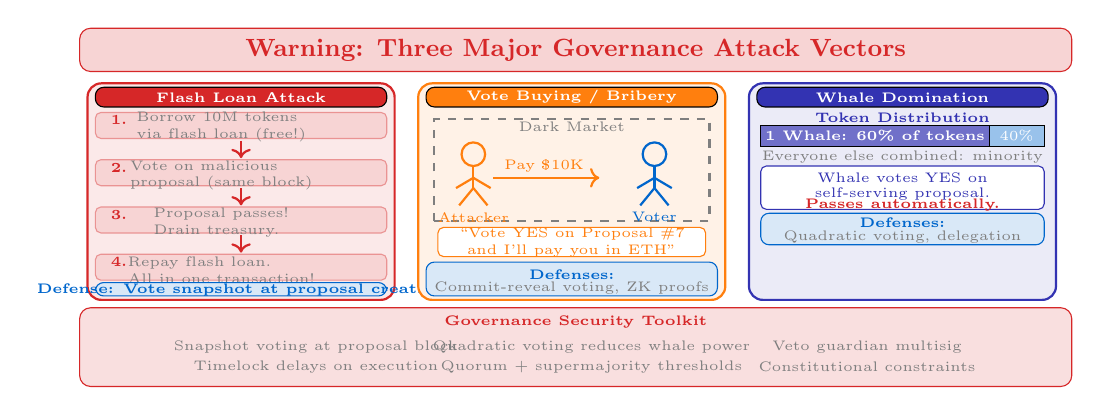
\begin{tikzpicture}
  % Title banner
  \draw[fill=mlred!20, draw=mlred, rounded corners=4pt] (0.0,4.3) rectangle (12.6,4.85);
  \node[font=\small\bfseries, mlred, align=center] at (6.3,4.57) {Warning: Three Major Governance Attack Vectors};

  % --- Attack 1: Flash Loan Attack ---
  \draw[fill=mlred!10, draw=mlred, rounded corners=5pt, thick] (0.1,1.4) rectangle (4.0,4.15);
  \draw[fill=mlred, rounded corners=3pt] (0.2,3.85) rectangle (3.9,4.1);
  \node[font=\tiny\bfseries, white, align=center] at (2.05,3.97) {Flash Loan Attack};

  % Step boxes
  \draw[fill=mlred!20, draw=mlred!50, rounded corners=2pt] (0.2,3.45) rectangle (3.9,3.78);
  \node[font=\tiny\bfseries, mlred] at (0.5,3.68) {1.};
  \node[font=\tiny, mlgray, align=left] at (1.8,3.6) {Borrow 10M tokens\\via flash loan (free!)};
  \draw[->, thick, mlred] (2.05,3.42) -- (2.05,3.2);
  \draw[fill=mlred!20, draw=mlred!50, rounded corners=2pt] (0.2,2.85) rectangle (3.9,3.18);
  \node[font=\tiny\bfseries, mlred] at (0.5,3.08) {2.};
  \node[font=\tiny, mlgray, align=left] at (1.8,2.98) {Vote on malicious\\proposal (same block)};
  \draw[->, thick, mlred] (2.05,2.82) -- (2.05,2.6);
  \draw[fill=mlred!20, draw=mlred!50, rounded corners=2pt] (0.2,2.25) rectangle (3.9,2.58);
  \node[font=\tiny\bfseries, mlred] at (0.5,2.48) {3.};
  \node[font=\tiny, mlgray, align=left] at (1.8,2.38) {Proposal passes!\\Drain treasury.};
  \draw[->, thick, mlred] (2.05,2.22) -- (2.05,2.0);
  \draw[fill=mlred!20, draw=mlred!50, rounded corners=2pt] (0.2,1.65) rectangle (3.9,1.98);
  \node[font=\tiny\bfseries, mlred] at (0.5,1.88) {4.};
  \node[font=\tiny, mlgray, align=left] at (1.8,1.78) {Repay flash loan.\\All in one transaction!};

  \draw[fill=mlblue!15, draw=mlblue, rounded corners=3pt] (0.2,1.45) rectangle (3.9,1.62);
  \node[font=\tiny\bfseries, mlblue, align=center] at (2.05,1.53) {Defense: Vote snapshot at proposal creation};

  % --- Attack 2: Vote Buying ---
  \draw[fill=mlorange!10, draw=mlorange, rounded corners=5pt, thick] (4.3,1.4) rectangle (8.2,4.15);
  \draw[fill=mlorange, rounded corners=3pt] (4.4,3.85) rectangle (8.1,4.1);
  \node[font=\tiny\bfseries, white, align=center] at (6.25,3.97) {Vote Buying / Bribery};

  % Diagram
  \draw[mlgray, dashed, thick] (4.5,2.4) rectangle (8.0,3.7);
  \node[font=\tiny, mlgray, align=center] at (6.25,3.6) {Dark Market};
  % Attacker
  \draw[mlorange,thick] (5.0,3.25) circle (0.15);
  \draw[mlorange,thick] (5.0,3.1) -- (5.0,2.82);
  \draw[mlorange,thick] (5.0,2.95) -- (4.78,2.82);
  \draw[mlorange,thick] (5.0,2.95) -- (5.22,2.82);
  \draw[mlorange,thick] (5.0,2.82) -- (4.82,2.6);
  \draw[mlorange,thick] (5.0,2.82) -- (5.18,2.6);
  \node[font=\tiny, mlorange] at (5.0,2.45) {Attacker};
  \draw[->, thick, mlorange] (5.25,2.95) -- (6.6,2.95);
  \node[font=\tiny, mlorange, align=center] at (5.9,3.1) {Pay \$10K};
  % Voter
  \draw[mlblue,thick] (7.3,3.25) circle (0.15);
  \draw[mlblue,thick] (7.3,3.1) -- (7.3,2.82);
  \draw[mlblue,thick] (7.3,2.95) -- (7.08,2.82);
  \draw[mlblue,thick] (7.3,2.95) -- (7.52,2.82);
  \draw[mlblue,thick] (7.3,2.82) -- (7.12,2.6);
  \draw[mlblue,thick] (7.3,2.82) -- (7.48,2.6);
  \node[font=\tiny, mlblue] at (7.3,2.45) {Voter};
  \draw[fill=white, draw=mlorange, rounded corners=2pt] (4.55,1.95) rectangle (7.95,2.32);
  \node[font=\tiny, mlorange, align=center] at (6.25,2.13) {``Vote YES on Proposal \#7\\and I'll pay you in ETH''};

  \draw[fill=mlblue!15, draw=mlblue, rounded corners=3pt] (4.4,1.45) rectangle (8.1,1.88);
  \node[font=\tiny\bfseries, mlblue, align=center] at (6.25,1.72) {Defenses:};
  \node[font=\tiny, mlgray, align=center] at (6.25,1.55) {Commit-reveal voting, ZK proofs};

  % --- Attack 3: Whale Domination ---
  \draw[fill=mlpurple!10, draw=mlpurple, rounded corners=5pt, thick] (8.5,1.4) rectangle (12.4,4.15);
  \draw[fill=mlpurple, rounded corners=3pt] (8.6,3.85) rectangle (12.3,4.1);
  \node[font=\tiny\bfseries, white, align=center] at (10.45,3.97) {Whale Domination};

  % Token distribution bar
  \node[font=\tiny\bfseries, mlpurple, align=center] at (10.45,3.72) {Token Distribution};
  \draw[fill=mlpurple!70] (8.65,3.35) rectangle (11.55,3.62);
  \node[font=\tiny\bfseries, white, align=center] at (10.1,3.48) {1 Whale: 60\% of tokens};
  \draw[fill=mlblue!40] (11.55,3.35) rectangle (12.25,3.62);
  \node[font=\tiny, white, align=center] at (11.9,3.48) {40\%};
  \node[font=\tiny, mlgray, align=center] at (10.45,3.22) {Everyone else combined: minority};

  \draw[fill=white, draw=mlpurple, rounded corners=2pt] (8.65,2.55) rectangle (12.25,3.1);
  \node[font=\tiny, mlpurple, align=center] at (10.45,2.95) {Whale votes YES on};
  \node[font=\tiny, mlpurple, align=center] at (10.45,2.75) {self-serving proposal.};
  \node[font=\tiny\bfseries, mlred, align=center] at (10.45,2.6) {Passes automatically.};

  \draw[fill=mlblue!15, draw=mlblue, rounded corners=3pt] (8.65,2.1) rectangle (12.25,2.5);
  \node[font=\tiny\bfseries, mlblue, align=center] at (10.45,2.38) {Defenses:};
  \node[font=\tiny, mlgray, align=center] at (10.45,2.2) {Quadratic voting, delegation};

  % Bottom summary
  \draw[fill=mlred!15, draw=mlred, rounded corners=4pt] (0.0,0.3) rectangle (12.6,1.3);
  \node[font=\tiny\bfseries, mlred, align=center] at (6.3,1.12) {Governance Security Toolkit};
  \node[font=\tiny, mlgray, align=center] at (3.0,0.8) {Snapshot voting at proposal block};
  \node[font=\tiny, mlgray, align=center] at (3.0,0.55) {Timelock delays on execution};
  \node[font=\tiny, mlgray, align=center] at (6.5,0.8) {Quadratic voting reduces whale power};
  \node[font=\tiny, mlgray, align=center] at (6.5,0.55) {Quorum + supermajority thresholds};
  \node[font=\tiny, mlgray, align=center] at (10.0,0.8) {Veto guardian multisig};
  \node[font=\tiny, mlgray, align=center] at (10.0,0.55) {Constitutional constraints};
\end{tikzpicture}

\bottomnote{Governance attacks are not theoretical -- flash loan governance attacks have drained millions. Defense requires: vote snapshots, timelocks, quadratic voting, and quorum requirements.}
\end{frame}

% Frame 9: Famous DAOs
\begin{frame}{Famous DAOs: Real-World Examples}
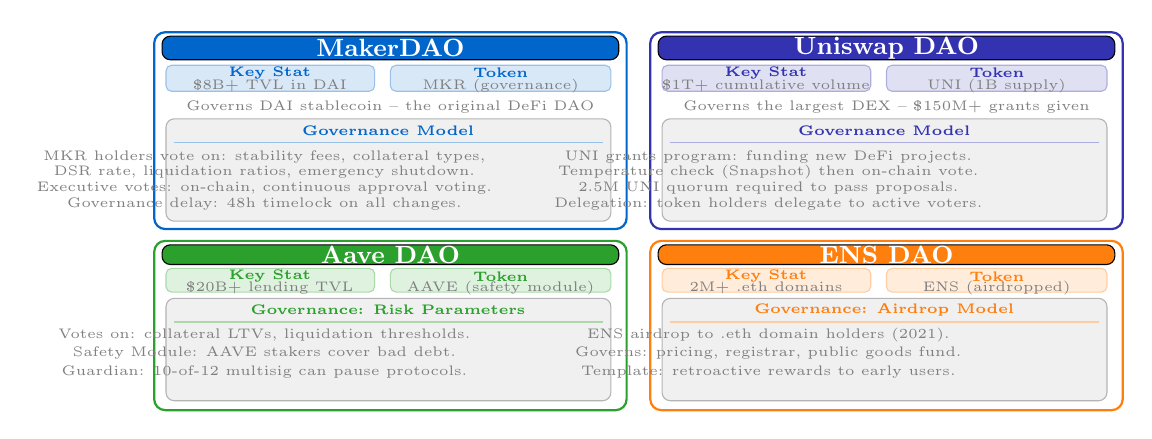
\begin{tikzpicture}
  % 2x2 grid of panels
  % Panel 1: MakerDAO (top-left)
  \draw[thick, mlblue, rounded corners=4pt] (0.1,2.4) rectangle (6.1,4.9);
  \draw[fill=mlblue, rounded corners=3pt] (0.2,4.55) rectangle (6.0,4.85);
  \node[font=\small\bfseries, white, align=center] at (3.1,4.7) {MakerDAO};
  % Stats
  \draw[fill=mlblue!15, draw=mlblue!40, rounded corners=2pt] (0.25,4.15) rectangle (2.9,4.48);
  \node[font=\tiny\bfseries, mlblue, align=center] at (1.57,4.38) {Key Stat};
  \node[font=\tiny, mlgray, align=center] at (1.57,4.22) {\$8B+ TVL in DAI};
  \draw[fill=mlblue!15, draw=mlblue!40, rounded corners=2pt] (3.1,4.15) rectangle (5.9,4.48);
  \node[font=\tiny\bfseries, mlblue, align=center] at (4.5,4.38) {Token};
  \node[font=\tiny, mlgray, align=center] at (4.5,4.22) {MKR (governance)};
  % Description
  \node[font=\tiny, mlgray, align=center] at (3.1,3.95) {Governs DAI stablecoin -- the original DeFi DAO};
  % Governance model
  \draw[fill=lightgray, draw=midgray, rounded corners=3pt] (0.25,2.5) rectangle (5.9,3.8);
  \node[font=\tiny\bfseries, mlblue, align=center] at (3.07,3.65) {Governance Model};
  \draw[mlblue!40, thin] (0.35,3.5) -- (5.8,3.5);
  \node[font=\tiny, mlgray, align=left] at (1.5,3.32) {MKR holders vote on: stability fees, collateral types,};
  \node[font=\tiny, mlgray, align=left] at (1.5,3.12) {DSR rate, liquidation ratios, emergency shutdown.};
  \node[font=\tiny, mlgray, align=left] at (1.5,2.92) {Executive votes: on-chain, continuous approval voting.};
  \node[font=\tiny, mlgray, align=left] at (1.5,2.72) {Governance delay: 48h timelock on all changes.};

  % Panel 2: Uniswap (top-right)
  \draw[thick, mlpurple, rounded corners=4pt] (6.4,2.4) rectangle (12.4,4.9);
  \draw[fill=mlpurple, rounded corners=3pt] (6.5,4.55) rectangle (12.3,4.85);
  \node[font=\small\bfseries, white, align=center] at (9.4,4.7) {Uniswap DAO};
  \draw[fill=mlpurple!15, draw=mlpurple!40, rounded corners=2pt] (6.55,4.15) rectangle (9.2,4.48);
  \node[font=\tiny\bfseries, mlpurple, align=center] at (7.87,4.38) {Key Stat};
  \node[font=\tiny, mlgray, align=center] at (7.87,4.22) {\$1T+ cumulative volume};
  \draw[fill=mlpurple!15, draw=mlpurple!40, rounded corners=2pt] (9.4,4.15) rectangle (12.2,4.48);
  \node[font=\tiny\bfseries, mlpurple, align=center] at (10.8,4.38) {Token};
  \node[font=\tiny, mlgray, align=center] at (10.8,4.22) {UNI (1B supply)};
  \node[font=\tiny, mlgray, align=center] at (9.4,3.95) {Governs the largest DEX -- \$150M+ grants given};
  \draw[fill=lightgray, draw=midgray, rounded corners=3pt] (6.55,2.5) rectangle (12.2,3.8);
  \node[font=\tiny\bfseries, mlpurple, align=center] at (9.37,3.65) {Governance Model};
  \draw[mlpurple!40, thin] (6.65,3.5) -- (12.1,3.5);
  \node[font=\tiny, mlgray, align=left] at (7.9,3.32) {UNI grants program: funding new DeFi projects.};
  \node[font=\tiny, mlgray, align=left] at (7.9,3.12) {Temperature check (Snapshot) then on-chain vote.};
  \node[font=\tiny, mlgray, align=left] at (7.9,2.92) {2.5M UNI quorum required to pass proposals.};
  \node[font=\tiny, mlgray, align=left] at (7.9,2.72) {Delegation: token holders delegate to active voters.};

  % Panel 3: Aave (bottom-left)
  \draw[thick, mlgreen, rounded corners=4pt] (0.1,0.1) rectangle (6.1,2.25);
  \draw[fill=mlgreen, rounded corners=3pt] (0.2,1.95) rectangle (6.0,2.2);
  \node[font=\small\bfseries, white, align=center] at (3.1,2.07) {Aave DAO};
  \draw[fill=mlgreen!15, draw=mlgreen!40, rounded corners=2pt] (0.25,1.6) rectangle (2.9,1.9);
  \node[font=\tiny\bfseries, mlgreen, align=center] at (1.57,1.8) {Key Stat};
  \node[font=\tiny, mlgray, align=center] at (1.57,1.65) {\$20B+ lending TVL};
  \draw[fill=mlgreen!15, draw=mlgreen!40, rounded corners=2pt] (3.1,1.6) rectangle (5.9,1.9);
  \node[font=\tiny\bfseries, mlgreen, align=center] at (4.5,1.8) {Token};
  \node[font=\tiny, mlgray, align=center] at (4.5,1.65) {AAVE (safety module)};
  \draw[fill=lightgray, draw=midgray, rounded corners=3pt] (0.25,0.22) rectangle (5.9,1.52);
  \node[font=\tiny\bfseries, mlgreen, align=center] at (3.07,1.37) {Governance: Risk Parameters};
  \draw[mlgreen!40, thin] (0.35,1.22) -- (5.8,1.22);
  \node[font=\tiny, mlgray, align=left] at (1.5,1.05) {Votes on: collateral LTVs, liquidation thresholds.};
  \node[font=\tiny, mlgray, align=left] at (1.5,0.82) {Safety Module: AAVE stakers cover bad debt.};
  \node[font=\tiny, mlgray, align=left] at (1.5,0.58) {Guardian: 10-of-12 multisig can pause protocols.};

  % Panel 4: ENS DAO (bottom-right)
  \draw[thick, mlorange, rounded corners=4pt] (6.4,0.1) rectangle (12.4,2.25);
  \draw[fill=mlorange, rounded corners=3pt] (6.5,1.95) rectangle (12.3,2.2);
  \node[font=\small\bfseries, white, align=center] at (9.4,2.07) {ENS DAO};
  \draw[fill=mlorange!15, draw=mlorange!40, rounded corners=2pt] (6.55,1.6) rectangle (9.2,1.9);
  \node[font=\tiny\bfseries, mlorange, align=center] at (7.87,1.8) {Key Stat};
  \node[font=\tiny, mlgray, align=center] at (7.87,1.65) {2M+ .eth domains};
  \draw[fill=mlorange!15, draw=mlorange!40, rounded corners=2pt] (9.4,1.6) rectangle (12.2,1.9);
  \node[font=\tiny\bfseries, mlorange, align=center] at (10.8,1.8) {Token};
  \node[font=\tiny, mlgray, align=center] at (10.8,1.65) {ENS (airdropped)};
  \draw[fill=lightgray, draw=midgray, rounded corners=3pt] (6.55,0.22) rectangle (12.2,1.52);
  \node[font=\tiny\bfseries, mlorange, align=center] at (9.37,1.37) {Governance: Airdrop Model};
  \draw[mlorange!40, thin] (6.65,1.22) -- (12.1,1.22);
  \node[font=\tiny, mlgray, align=left] at (7.9,1.05) {ENS airdrop to .eth domain holders (2021).};
  \node[font=\tiny, mlgray, align=left] at (7.9,0.82) {Governs: pricing, registrar, public goods fund.};
  \node[font=\tiny, mlgray, align=left] at (7.9,0.58) {Template: retroactive rewards to early users.};
\end{tikzpicture}

\bottomnote{MakerDAO, Uniswap, Aave, and ENS DAO are among the most successful DAOs, collectively governing billions in assets and setting governance design patterns for the industry.}
\end{frame}

% Frame 10: Key Takeaways
\begin{frame}{Key Takeaways}
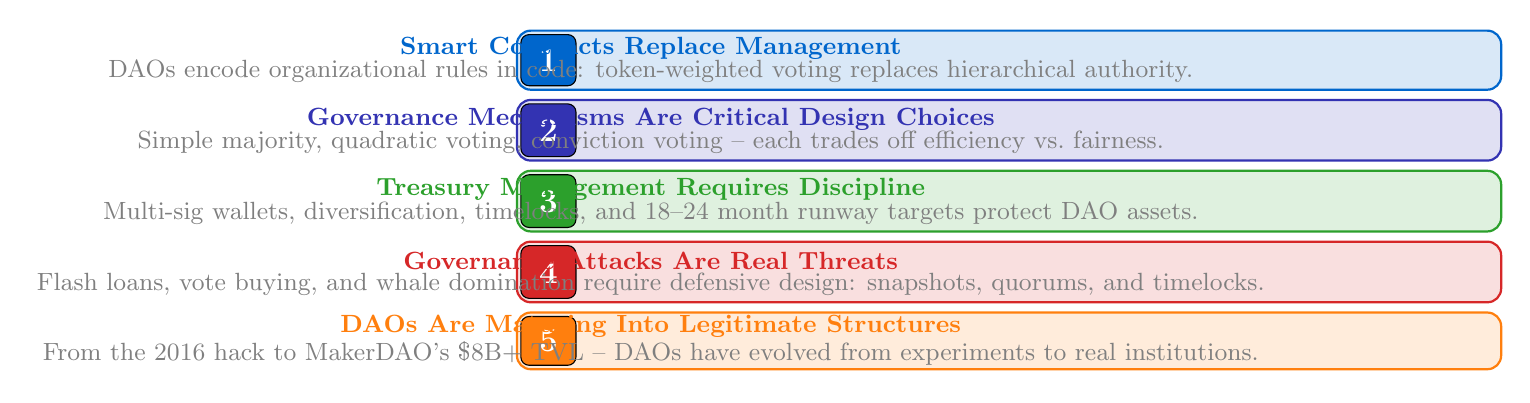
\begin{tikzpicture}
  % Takeaway 1
  \draw[fill=mlblue!15, draw=mlblue, rounded corners=5pt, thick] (0.0,3.55) rectangle (12.5,4.3);
  \draw[fill=mlblue, rounded corners=3pt] (0.05,3.6) rectangle (0.75,4.25);
  \node[font=\large\bfseries, white, align=center] at (0.4,3.92) {1};
  \node[font=\small\bfseries, mlblue, align=left] at (1.7,4.08) {Smart Contracts Replace Management};
  \node[font=\small, mlgray, align=left] at (1.7,3.78) {DAOs encode organizational rules in code: token-weighted voting replaces hierarchical authority.};

  % Takeaway 2
  \draw[fill=mlpurple!15, draw=mlpurple, rounded corners=5pt, thick] (0.0,2.65) rectangle (12.5,3.42);
  \draw[fill=mlpurple, rounded corners=3pt] (0.05,2.7) rectangle (0.75,3.37);
  \node[font=\large\bfseries, white, align=center] at (0.4,3.03) {2};
  \node[font=\small\bfseries, mlpurple, align=left] at (1.7,3.18) {Governance Mechanisms Are Critical Design Choices};
  \node[font=\small, mlgray, align=left] at (1.7,2.88) {Simple majority, quadratic voting, conviction voting -- each trades off efficiency vs.\ fairness.};

  % Takeaway 3
  \draw[fill=mlgreen!15, draw=mlgreen, rounded corners=5pt, thick] (0.0,1.75) rectangle (12.5,2.52);
  \draw[fill=mlgreen, rounded corners=3pt] (0.05,1.8) rectangle (0.75,2.47);
  \node[font=\large\bfseries, white, align=center] at (0.4,2.13) {3};
  \node[font=\small\bfseries, mlgreen, align=left] at (1.7,2.28) {Treasury Management Requires Discipline};
  \node[font=\small, mlgray, align=left] at (1.7,1.98) {Multi-sig wallets, diversification, timelocks, and 18--24 month runway targets protect DAO assets.};

  % Takeaway 4
  \draw[fill=mlred!15, draw=mlred, rounded corners=5pt, thick] (0.0,0.85) rectangle (12.5,1.62);
  \draw[fill=mlred, rounded corners=3pt] (0.05,0.9) rectangle (0.75,1.57);
  \node[font=\large\bfseries, white, align=center] at (0.4,1.23) {4};
  \node[font=\small\bfseries, mlred, align=left] at (1.7,1.38) {Governance Attacks Are Real Threats};
  \node[font=\small, mlgray, align=left] at (1.7,1.08) {Flash loans, vote buying, and whale domination require defensive design: snapshots, quorums, and timelocks.};

  % Takeaway 5
  \draw[fill=mlorange!15, draw=mlorange, rounded corners=5pt, thick] (0.0,0.0) rectangle (12.5,0.72);
  \draw[fill=mlorange, rounded corners=3pt] (0.05,0.05) rectangle (0.75,0.67);
  \node[font=\large\bfseries, white, align=center] at (0.4,0.36) {5};
  \node[font=\small\bfseries, mlorange, align=left] at (1.7,0.55) {DAOs Are Maturing Into Legitimate Structures};
  \node[font=\small, mlgray, align=left] at (1.7,0.2) {From the 2016 hack to MakerDAO's \$8B+ TVL -- DAOs have evolved from experiments to real institutions.};
\end{tikzpicture}

\vspace{0.05cm}

\begin{tikzpicture}
  \draw[fill=mlpurple, rounded corners=4pt] (0,0) rectangle (12.5,0.52);
  \node[font=\small\bfseries, white, align=center] at (6.25,0.26) {Next: Governance Mechanisms -- Quadratic Voting, Conviction Voting, and DAO Legal Wrappers};
\end{tikzpicture}

\bottomnote{DAOs are a new organizational primitive: transparent, borderless, and code-governed. Understanding their strengths and failure modes is essential for any blockchain practitioner.}
\end{frame}

\end{document}
